\documentclass{article}

%opening
\title{Simulating Rayleigh Fading MIMO Channel Capacity\thanks{Simulation code uploaded on https://github.com/lightwick/ICS$\textunderscore$project/tree/main/Spatial$\textunderscore$Diversity}\\
\large Project \#5}
\author{Intelligent Communication Systems (ICS) Lab.\\노용재}
\date{Winter Intern Seminar (2023-1)}

\usepackage{kotex} % korean
\usepackage[margin=1in]{geometry} % 둘레 margin
\usepackage{matlab-prettifier}
\usepackage{amsmath}
\usepackage{graphicx} % image
\usepackage{subcaption}
\usepackage{xcolor} % for coloring text
\usepackage{amssymb} % because, therefore symbol
\usepackage{float}
\usepackage{wrapfig}
\usepackage{booktabs}
\usepackage{changepage}

\newcommand{\bd}{\textbf} % bold
\providecommand{\abs}[1]{\lvert#1\rvert}
\graphicspath{{./img/}}
\newcommand{\sgn}{\operatorname{sgn}}
\begin{document}

\maketitle
\tableofcontents
\vspace{0.5cm}
\hrule
\vspace{0.5cm}

\section{Theory}
\subsection{Channel Unknown to the Transmitter}
특이값 분해(Singular Value Decomposition;SVD)에 따르면 모든 행렬은 $U\Sigma V^H$로 분해할 수 있다.
이때, $\Sigma$는 대각 성분이 음수가 아닌 실수로만 이루어진 대각행렬이며 $U$와 $V$는 직교행렬이다.\\
임의의 행렬 $H$에 대해 다음이 성립한다.
\begin{gather}
H=U\Sigma V^H\\
H^H = V \Sigma^H U^H\\
\begin{split}
HH^H&=(U\Sigma V^H)(V \Sigma^H U^H)\\
&=U\Sigma \Sigma^H U^H\\
&=U\Sigma^2 U^H (\because \Sigma=\Sigma^H)\\
\end{split}
\end{gather}
\hspace{10cm}$\therefore HH^H=U\Sigma U^H$\\

직교행렬 $Q$에 의해 $HH^H=Q\Sigma Q^H$와 같이 나타낼 수 있다. 이 특성을 이용하여 \textsl{Capacity}, $C$를 다음과 같이 나타낼 수 있다.
% $\Sigma^H = \begin{bmatrix} \sigma_1 & 0 & \cdots & 0 \\ 0 & \sigma_2 & \cdots & 0 \\ \vdots & \vdots & \ddots & \vdots \\ 0 & 0 & \cdots & \sigma_r \\ 0 & 0 & \cdots & 0 \\ \vdots & \vdots & \ddots & \vdots \\ 0 & 0 & \cdots & 0 \end{bmatrix}^H = \begin{bmatrix} \sigma_1^* & 0 & \cdots & 0 \\ 0 & \sigma_2^* & \cdots & 0 \\ \vdots & \vdots & \ddots & \vdots \\ 0 & 0 & \cdots & \sigma_r^* \\ 0 & 0 & \cdots & 0 \\ \vdots & \vdots & \ddots & \vdots \\ 0 & 0 & \cdots & 0 \end{bmatrix}$

\begin{gather}
\begin{split}
C &=\log_2 \det(I_{N_R}+\frac{E_S}{N_T N_0}HH^H)\\
&=\log_2 \det(I_{N_R}+\frac{E_S}{N_T N_0}Q\Lambda Q^H)\\
&=\log_2 \det(I_{N_R}+\frac{E_S}{N_T N_0}Q^HQ\Lambda)\ (\because \det(I+AB)=\det(I+BA))\\
&=\log_2 \det(I_{N_R}+\frac{E_S}{N_T N_0}\Lambda)\ (\because Q^HQ=I)\\
&=\sum_{i=1}^r\log_2 (1+\frac{E_S}{N_T N_0}\lambda_i)\\
\end{split}
\end{gather}

\subsection{Channel Known to the Transmitter; Waterpouring Algorithm}
$r$개의 sub-channel이 있을 때, $\sum_{i=1}^r\gamma_i=N_T$라 하자.
\begin{gather}
\begin{split}
C &=\sum_{i=1}^r\log_2 (1+\frac{E_S\gamma_i}{N_T N_0}\lambda_i)\\
\end{split}
\end{gather}
$r$개의 sub-channel에 따라 전력을 적절히 분배하여 Capacity를 최대화하려 한다.\\
\\
Lagrangian method를 사용하여 $\sum_{i=1}^r\gamma_i=N_T$일 때, $C =\sum_{i=1}^r\log_2 (1+\frac{E_S\gamma_i}{N_T N_0}\lambda_i)$의 값을 최대화하자.\\
\\
\bd{Lagrangian Method}
\begin{gather}
\mathcal{L}(\gamma_1, ..., \gamma_{r}, \theta)=\sum_{i=1}^r\log_2 (1+\frac{E_S\gamma_i}{N_T N_0}\lambda_i)-\theta(\sum_{i=1}^r\gamma_i-N_T)
\end{gather}
Lagrangian이 식(6)과 같을 때 $\nabla\mathcal{L} = \vec{0}$을 만족하여야 한다. ($\rho=\frac{E_S}{N_0}$)
\begin{gather}
\nabla\mathcal{L}=
\begin{bmatrix}
\frac{\partial \mathcal{L}}{\partial \gamma_1}\\
\vdots\\
\frac{\partial \mathcal{L}}{\partial \gamma_r}\\
\frac{\partial \mathcal{L}}{\partial \theta}
\end{bmatrix}
=
\begin{bmatrix}
\frac{1}{(1+\frac{\gamma_1}{N_T}\rho\lambda_1)\ln2}\frac{\rho\lambda_1}{N_T}-\theta\\
\vdots\\
\frac{1}{(1+\frac{\gamma_r}{N_T}\rho\lambda_r)\ln2}\frac{\rho\lambda_r}{N_T}-\theta\\
\sum_{i=1}^r\gamma_i-N_T
\end{bmatrix}
=\vec{0}
\end{gather}
즉, 모든 $i\ (i=1,2..,r)$에 대해 다음을 만족한다.
\begin{gather}
\frac{1}{(1+\frac{\gamma_i}{N_T}\rho\lambda_i)\ln2}\frac{\rho\lambda_i}{N_T}-\theta=0
\end{gather}
이를 정리하면,
\begin{gather}
\gamma_i=\frac{1}{\theta\ln2}-\frac{N_T}{\rho\lambda_i}
\end{gather}

\begin{gather}
\begin{split}
\sum_{i=1}^r\gamma_i-N_T &= \sum_{i=1}^r(\frac{1}{\theta\ln2}-\frac{N_T}{\rho\lambda_i})-N_T\\
&=\frac{r}{\theta\ln2}-\frac{N_T}{\rho}\sum_{i=1}^r\frac{1}{\lambda_i}-N_T
\end{split}\\
\frac{r}{\theta\ln2}-\frac{N_T}{\rho}\sum_{i=1}^r\frac{1}{\lambda_i}-N_T=0\\
\\
\frac{1}{\theta\ln2}=\frac{N_T}{r}(1+\frac{1}{\rho}\sum_{i=1}^r\frac{1}{\lambda_i})
\end{gather}
이를 식(9)에 대입하자.
\begin{gather}
\gamma_i = \frac{N_T}{r}(1+\frac{1}{\rho}\sum_{j=1}^r\frac{1}{\lambda_j}) - \frac{N_T}{\rho\lambda_i}
\end{gather}
\newpage
\section{Implementation}
\subsection{Channel Unknown to the Transmitter}
Capacity를 SNR에 따른 column vector로 정리하여 나타낸다.
\begin{adjustwidth}{-1.5cm}{-1.5cm}
\begin{lstlisting}[style=Matlab-editor, frame=single, numbers=left,]
function [EntireCapacity, ErgodicCapacity, OutageCapacity] = getCapcity_CU(Nr, Nt, EsN0_dB, iTotal)
    % EntireCapacity is a 'Column Vector'
    EntireCapacity = zeros(iTotal, length(EsN0_dB));
    ErgodicCapacity = zeros(length(EsN0_dB), 1);
    OutageCapacity = zeros(length(EsN0_dB), 1);
    
    EsN0 = db2pow(EsN0_dB);
    
    for EsN0_idx=1:length(EsN0_dB)
        %% Get Capacity array
        for iteration=1:iTotal
            H = (randn(Nr, Nt) + 1j * randn(Nr, Nt)) / sqrt(2); % Receiver x Transmitter
            Capacity = log2(det(eye(Nr)+EsN0(EsN0_idx)/Nt*H*H'));
            EntireCapacity(iteration, EsN0_idx) = Capacity;
        end
        
        %% Outage Capcity
        [cdf,x] = ecdf(EntireCapacity(:, EsN0_idx));
        [~, Outage_idx] = min(abs(cdf-0.1));
        OutageCapacity(EsN0_idx) = x(Outage_idx);
        
    end
    %% Ergodic Capcity
    ErgodicCapacity = real(mean(EntireCapacity))';
end
\end{lstlisting}
\end{adjustwidth}
\newpage
\subsection{Channel Known to the Transmitter}
Capacity를 SNR에 따른 column vector로 정리하여 나타낸다.
\begin{adjustwidth}{-1.5cm}{-1.5cm}
\begin{lstlisting}[style=Matlab-editor, frame=single, numbers=left,]
function [EntireCapacity, ErgodicCapacity, OutageCapacity] = getCapcity_CK(Nr, Nt, EsN0_dB, iTotal)
    % EntireCapacity is a 'Column Vector'
    EntireCapacity = zeros(iTotal, length(EsN0_dB));
    ErgodicCapacity = zeros(length(EsN0_dB), 1);
    OutageCapacity = zeros(length(EsN0_dB), 1);
    
    EsN0 = db2pow(EsN0_dB);
    
    for EsN0_idx=1:length(EsN0_dB)
        %% Get Capacity array
        for iteration=1:iTotal
            H = (randn(Nr, Nt) + 1j * randn(Nr, Nt)) / sqrt(2); % Receiver x Transmitter
            
            p = 1;
            [~,S,~] = svd(H);
            
            if min(size(S))==1
                EigenValues = S(1,1)^2;
            else
                EigenValues = diag(S).^2;
            end
            
            while true
                r = rank(H);
                PowerDistribution = Nt/(r-p+1)*(1+1/EsN0(EsN0_idx)*sum(1./EigenValues, 'all')) - Nt/EsN0(EsN0_idx)*(1./EigenValues);
                if PowerDistribution(r-p+1)>=0
                    break;
                else
                    p = p+1;
                    EigenValues(length(EigenValues))=[];
                end
            end
            Capacity = sum(log2(1+EsN0(EsN0_idx)/Nt * PowerDistribution.*EigenValues), 'all');
            EntireCapacity(iteration, EsN0_idx) = Capacity;
        end
        
        %% Outage Capcity
        [cdf,x] = ecdf(EntireCapacity(:, EsN0_idx));
        [~, Outage_idx] = min(abs(cdf-0.1));
        OutageCapacity(EsN0_idx) = x(Outage_idx);
    end
    %% Ergodic Capcity
    ErgodicCapacity = real(mean(EntireCapacity))';
end
\end{lstlisting}
\end{adjustwidth}

\section{결과 및 분석}
\subsection{Simulation Result}
\subsubsection{CDF of Capacity}
\bd{2x2 MIMO: $\boldsymbol{E_S$/$N_0}$=10dB}
\begin{figure}[H]
	\centering
	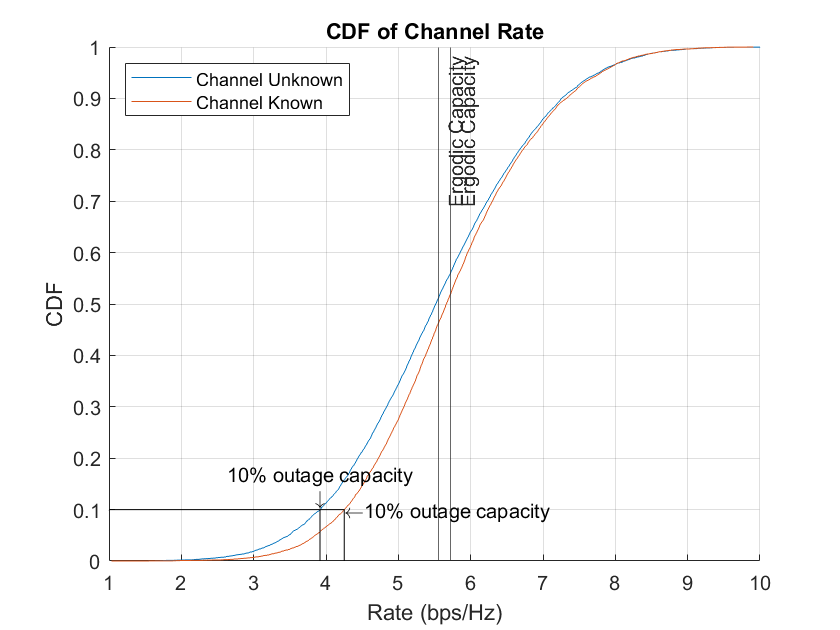
\includegraphics[width=.5\textwidth]{a.png}
	\caption{}
\end{figure}

\subsubsection{Capacity by Antenna Number}
\begin{figure}[H]
	\centering
	\begin{subfigure}{0.5\textwidth}
		\centerline{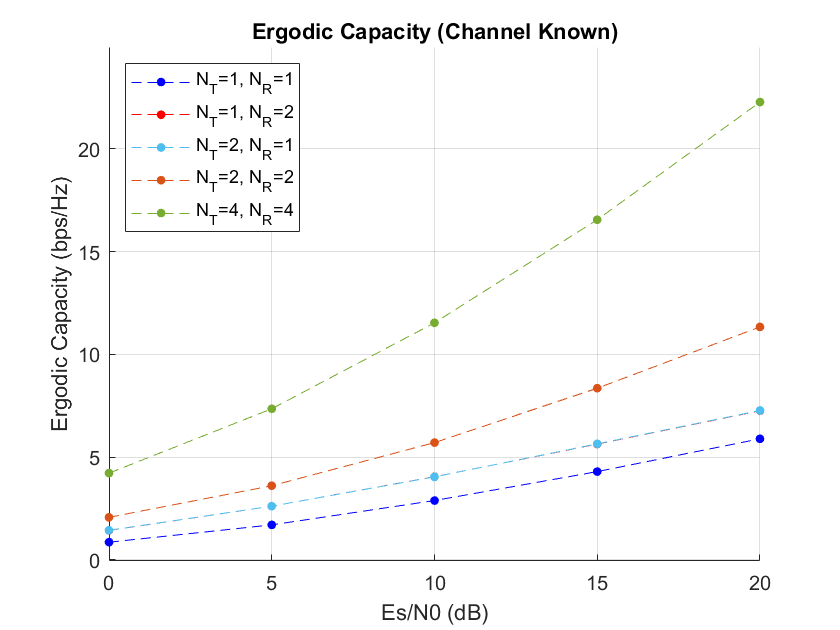
\includegraphics[width=1\textwidth]{b_ergodic_ck.png}}
		\caption{Channel Known to Transmitter}
	\end{subfigure}%
	\begin{subfigure}{0.5\textwidth}
		\centerline{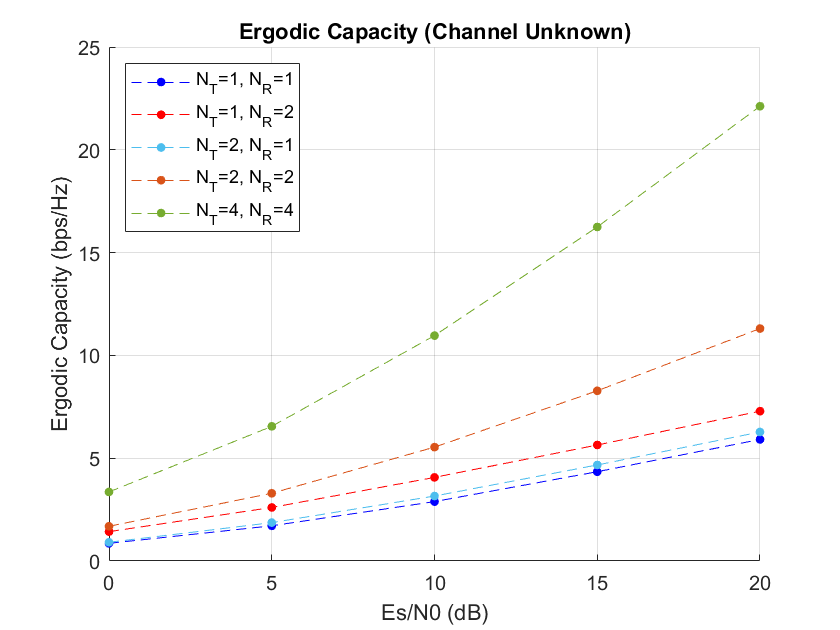
\includegraphics[width=1\textwidth]{b_ergodic_cu.png}}
		\caption{Channel Unknown to Transmitter}
	\end{subfigure}\\%
	\caption{Ergodic Capacity}
	\begin{subfigure}{0.5\textwidth}
		\centerline{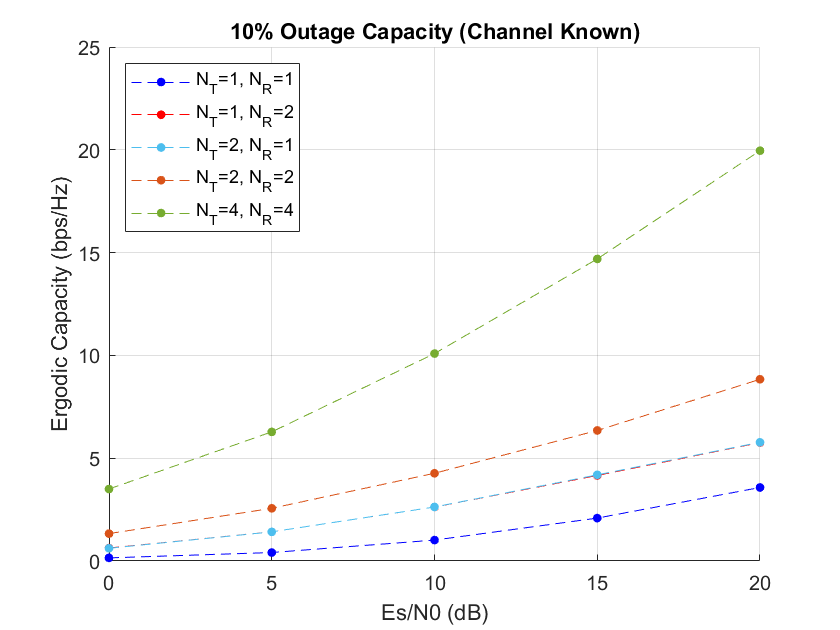
\includegraphics[width=1\textwidth]{b_outage_ck.png}}
		\caption{Channel Known to Transmitter}
	\end{subfigure}%
	\begin{subfigure}{0.5\textwidth}
		\centerline{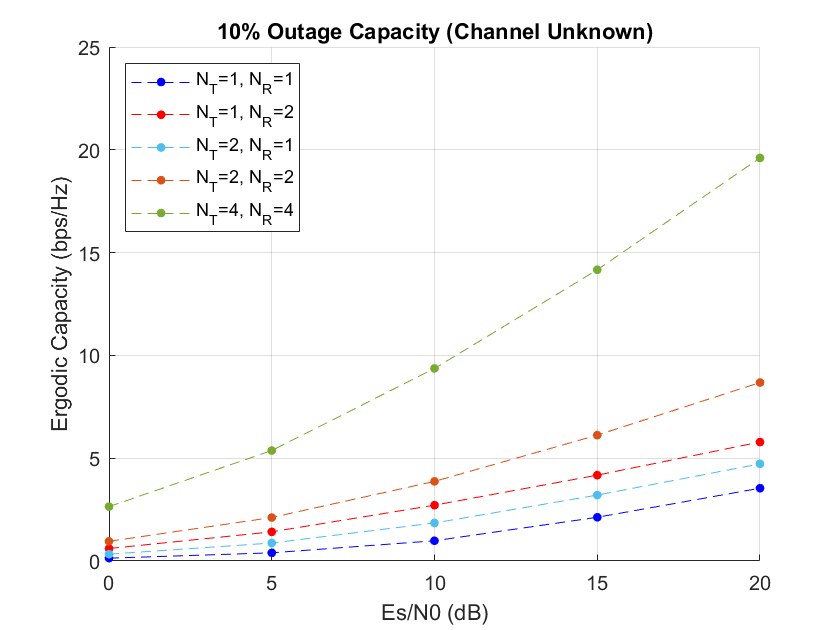
\includegraphics[width=1\textwidth]{b_outage_cu.png}}
		\caption{Channel Unknown to Transmitter}
	\end{subfigure}\\%
	\caption{10\% Outage Capacity}
\end{figure}
Channel Known의 경우, $N_T>N_R$($N_T=\alpha, N_R=\beta$)일 때의 \textsl{capacity}는 $N_T=\beta, N_R=\alpha$일 때의 \textsl{capacity}와 거의 일치하는 모습을 보였다.

\subsubsection{Ergodic Capacity by Channel Knowledge}
\begin{figure}[H]
	\centering
	\begin{subfigure}{0.5\textwidth}
		\centerline{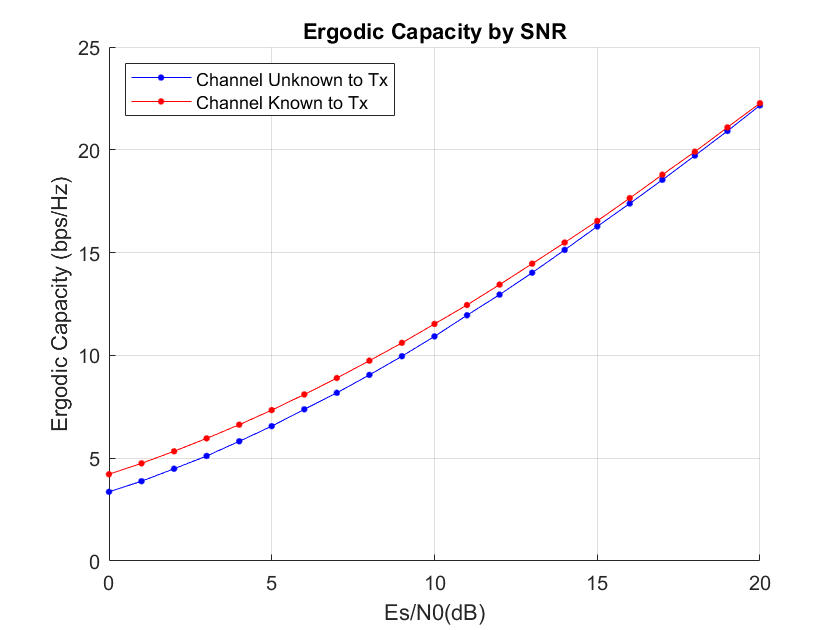
\includegraphics[width=1\textwidth]{c_ergodic.png}}
		\caption{4x4 MIMO}
	\end{subfigure}%
	\begin{subfigure}{0.5\textwidth}
		\centerline{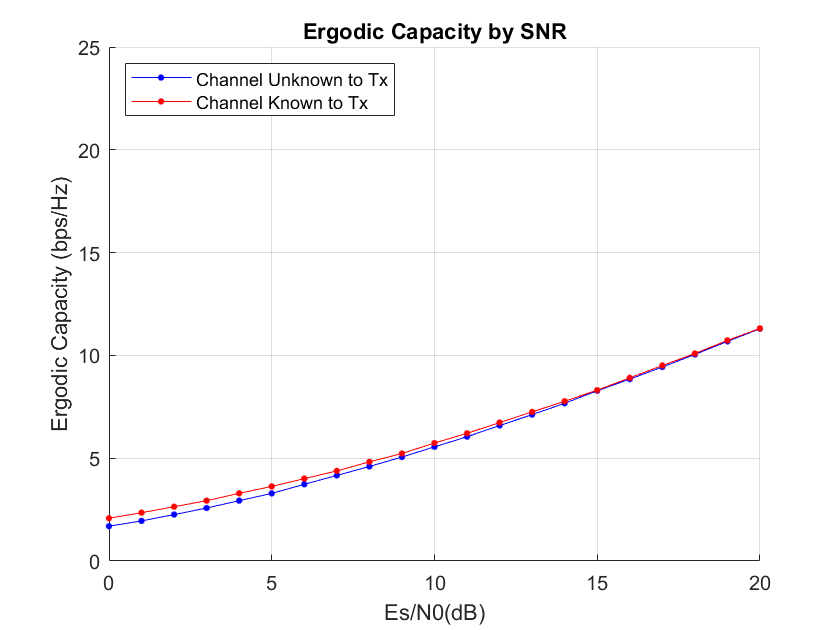
\includegraphics[width=1\textwidth]{c_ergodic_2x2.png}}
		\caption{2x2 MIMO}
	\end{subfigure}\\%
	\caption{}
\end{figure}

\subsection{CK, CU간 Capacity 차이 분석}
\begin{figure}[H]
	\centering
	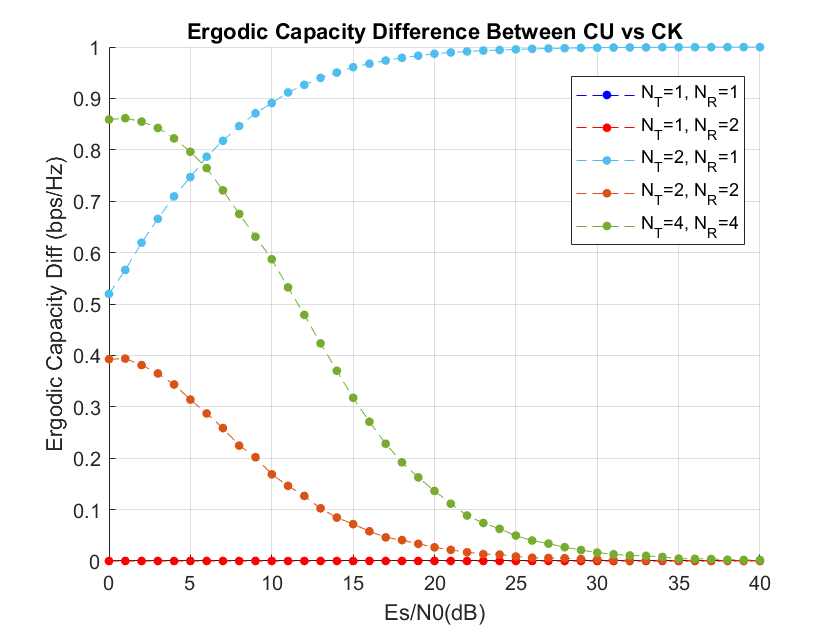
\includegraphics[width=.5\textwidth]{ergodic_diff.png}
	\caption{}
\end{figure}
\bd{Figure 5}는 transmitter가 channel에 대한 정보를 아는 경우와 모르는 경우 간의 capacity 차이를 나타낸 것이다.
$N_T=1, N_R=1$와 $N_T=1, N_R=2$일 때, 그 차이는 0이다. 그 외의 경우에는 모두 특정 값으로 수렴한다. 이것에 대해 분석해 보겠다.\\
이후 Channel에 대한 정보가 transmitter에게 있는 경우의 capacity는 $C_{CK}$, 없는 경우의 capacity는 $C_{CU}$이라 하겠다.

\subsubsection{SIMO에서의 Capacity; $\boldsymbol{C_{CK}-C_{CU}=0}$}
\begin{figure}[H]
	\centering
	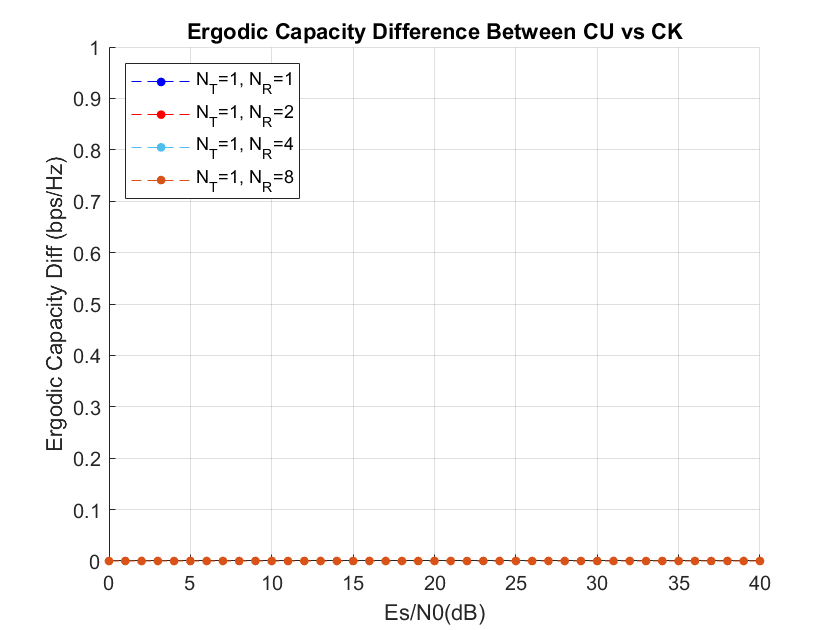
\includegraphics[width=.5\textwidth]{ergodic_simo.png}
	\caption{}
\end{figure}
\bd{Figure 6}를 보면 SISO와 SIMO의 경우에 $C_{CK}-C_{CU}=0$인 것을 확인할 수 있다. 즉, channel knowledge가 capacity에 영향을 미치지 않는다는 것을 알 수 있다.\\
\textsl{Channel Known case}인 Waterpouring algorithm의 식 (5)를 살펴보자. SIMO에서 $r=rank(H)=1$이다.이며 $\gamma_1=1$이다.
\begin{gather}
\begin{split}
C_{CK} &=\sum_{i=1}^r\log_2 (1+\frac{E_S\gamma_i}{N_T N_0}\lambda_i)\\
&=\sum_{i=1}^r\log_2 (1+\frac{E_S}{N_T N_0}\lambda_i)\\
&=C_{CU}
\end{split}
\end{gather}
즉, $C_{CK}=C_{CU}$이다.
\subsubsection{MISO에서 Capacity 차이 수렴; $\boldsymbol{C_{CK}-C_{CU}=\log_2{N_T}}$}
\begin{figure}[H]
	\centering
	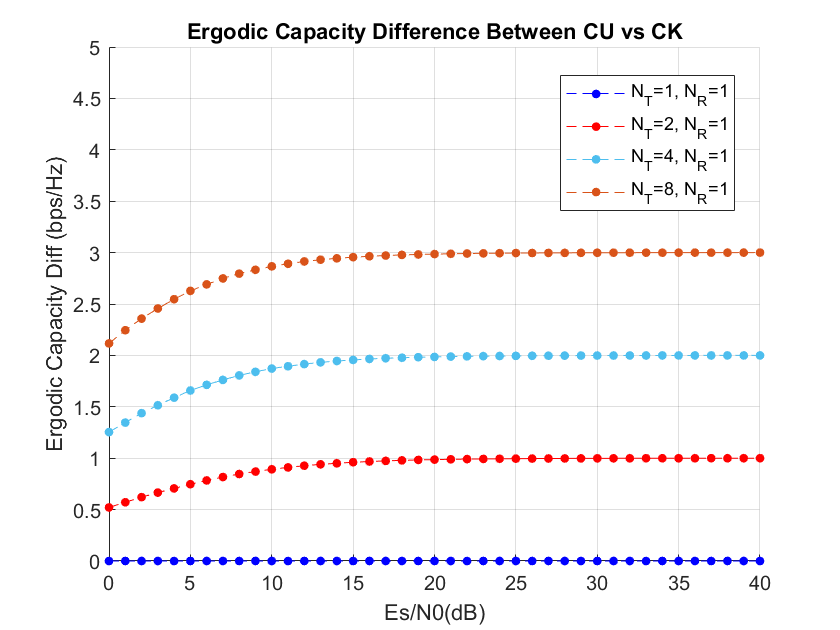
\includegraphics[width=.5\textwidth]{ergodic_diff_miso.png}
	\caption{}
\end{figure}
\bd{Figure 7}를 보면, $C_{CK}-C_{CU}=\log_2{N_T}$로 수렴하는 것을 볼 수 있다. MISO에서 $r=rank(H)=1$이다.
\begin{gather}
\begin{split}
\lim_{\rho\rightarrow\infty}(C_{CK}-C_{CU})&=\lim_{\rho\rightarrow\infty}(\log_2{(1+\frac{\gamma}{N_T}\rho\lambda_1)}-\log_2{(1+\frac{\rho}{N_T}\lambda_1}))\\
&=\lim_{\rho\rightarrow\infty}\log_2{\frac{1+\frac{\gamma_1}{N_T}\rho\lambda_1}{1+\frac{1}{N_T}\rho\lambda_1}}\\
&=\log_2{\gamma_1}\\
&=\log_2{N_T}
\end{split}
\end{gather}
\end{document}